\documentclass[10pt]{beamer}

\usetheme{metropolis}
%\metroset{background=dark}
%\usepackage{appendixnumberbeamer}
\usepackage{tikz}
\usepackage{fontawesome}
\usetikzlibrary{positioning}
\definecolor{cobaltBlue}{HTML}{38ACEC}
%\setbeamercolor{alerted text}{fg=cobaltBlue}
\usepackage{booktabs}
\usepackage[scale=2]{ccicons}

\usepackage{pgfplots}
\usepgfplotslibrary{dateplot}

\usepackage{xspace}

\newcommand{\lift}{\textsc{lift}\space}
\newcommand{\srcurl}[1]{\textcolor{blue}{\textit{#1}}}
\newcommand{\code}[1]{\textbf{\texttt{#1}}}

%\setbeamercolor*{structure}{bg=black,fg=white}


\title{Lift: The Language, The IR and Code Generation}
\date{April 2nd, 2018}
\author{\textbf{Naums Mogers}}
\institute{University of Edinburgh}

\begin{document}

\begin{frame}[plain,noframenumbering]
\maketitle
\end{frame}

\begin{frame}
\frametitle{Table of contents}
\begin{itemize}
	\item Lift -- An Intermediate Language
	\item Writing an Application
	\item Lift Intermediate Representation
	\item Lift Compilation
\end{itemize}
\end{frame}

\section{\lift -- An Intermediate Language}
\begin{frame}
\frametitle{Algorithmic Patterns}
    \begin{block}{}
        \begin{center}
            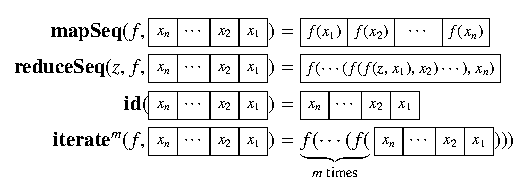
\includegraphics[width=.85\textwidth]{../images/algorithmic_patterns.pdf}
        \end{center}
    \end{block}
\end{frame}

\begin{frame}
\frametitle{Data Layout Patterns}
    \begin{block}{}
        \begin{center}
            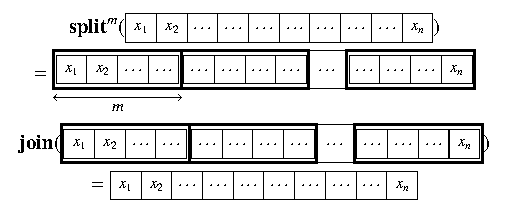
\includegraphics[width=.85\textwidth]{../images/data_layout_patterns1.pdf}
        \end{center}
    \end{block}
\begin{itemize}
	\item Do not perform any computation
	\item Reorganize the data layout (\code{View})
\end{itemize}
\end{frame}


\begin{frame}
\frametitle{Data Layout Patterns}
    \vspace{-.5cm}
    \begin{block}{}
        \begin{center}
            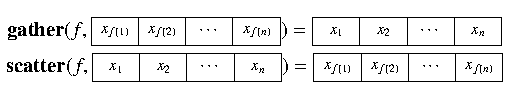
\includegraphics[width=.85\textwidth]{../images/data_layout_patterns2.pdf}
        \end{center}
        \vspace{-.5cm}
        \begin{center}
            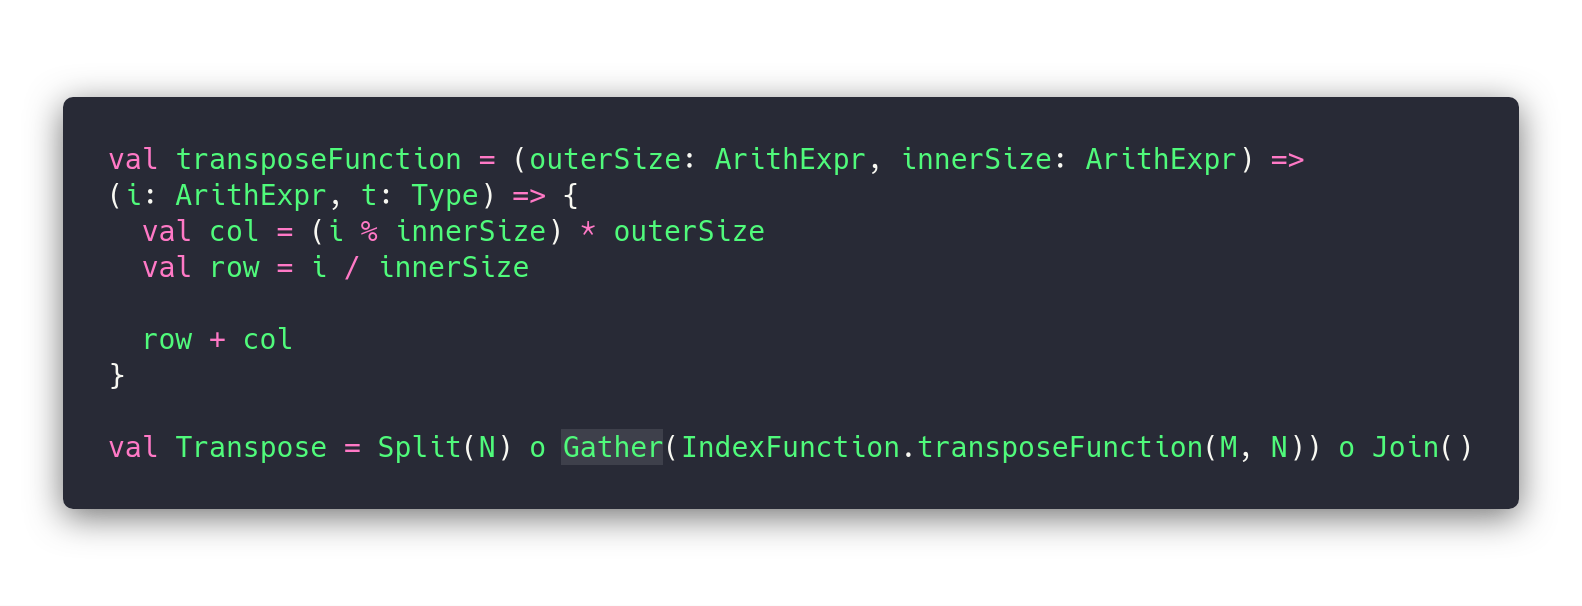
\includegraphics[width=.85\textwidth]{../images/gather.png}
        \end{center}
    \end{block}
    \vspace{-.5cm}
\begin{center}
	For examples of \code{Gather} and \code{Scatter} indexing functions, see \srcurl{src/main/ir/ast/package.scala}
\end{center}
\end{frame}

\begin{frame}
\frametitle{Data Layout Patterns}
    \begin{block}{}
        \begin{center}
            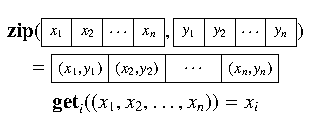
\includegraphics[width=.55\textwidth]{../images/data_layout_patterns3.pdf}
        \end{center}
        \begin{center}
            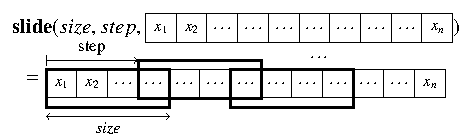
\includegraphics[width=.85\textwidth]{../images/data_layout_patterns4.pdf}
        \end{center}
    \end{block}
\end{frame}

\begin{frame}
\frametitle{Parallel Patterns}
\begin{columns}[onlytextwidth]
\begin{column}{0.45\textwidth}
\begin{itemize}
	\item \code{mapWrg$(0-2)$}
	\item \code{mapLcl$(0-2)$}
	\item \code{mapGlb$(0-2)$}
\end{itemize}
\end{column}
\begin{column}{0.45\textwidth}
\begin{itemize}	
	\item \code{mapWarp}
	\item \code{mapLane}
\end{itemize}
\end{column}
\end{columns}
\end{frame}

\begin{frame}
\frametitle{Address Space Patterns}
    \begin{block}{}
        \begin{center}
            
\includegraphics[width=.55\textwidth]{../images/address_space_patterns.pdf}
        \end{center}
        \begin{center}
            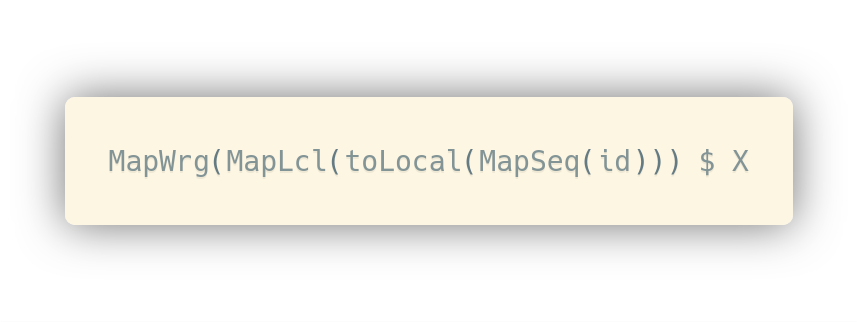
\includegraphics[width=.55\textwidth]{../images/toLocal.png}
        \end{center}
    \end{block}
\begin{itemize}
    \item These primitives decouple the decision of \textit{where} to store data from the decision of \textit{how} the data is produced.
\end{itemize}
\end{frame}

\begin{frame}
\frametitle{Vectorize Pattern}
    \begin{block}{}
        \begin{center}
            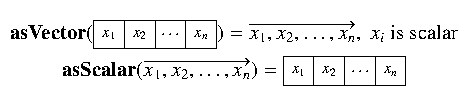
\includegraphics[width=.85\textwidth]{../images/vectorize_pattern.pdf}
        \end{center}
    \end{block}
\begin{itemize}
    \item During code generation, the \lift compiler transforms \textit{f} into a vectorized form using OpenCL built-in vectorized arithmetic operations whenever possible.
	\begin{itemize}
	    \item In other cases, \textit{f} is applied to each scalar in the vector.
    \end{itemize}
\end{itemize}
\end{frame}

\begin{frame}
\frametitle{Low-level IRs}
All \lift primitives are either:
\begin{itemize}
	\item High-level, capturing rich information about the algorithmic structure of programs
	\item Low-level and platform-specific (OpenCL, OpenCL for FPGAs, OpenMP, etc)
\end{itemize}
\end{frame}

\section{Writing an Application}

\begin{frame}
\frametitle{General Steps}
\begin{itemize}
    \item Determine input parameters 
    \item Initialise input data 
            \begin{itemize}
                \item If testing, initialise comparison data 
            \end{itemize}
    \item Craft or translate the algorithm of interest 
    \item Create an OpenCL kernel from your algorithm 
\end{itemize}
\end{frame}

\begin{frame}
\frametitle{Data Input to Lift Algorithms}
\begin{itemize}
    \item Lift can take in arrays or scalars as input parameters
            \vspace{-1.2cm}
\begin{block}{}
    \begin{center}
    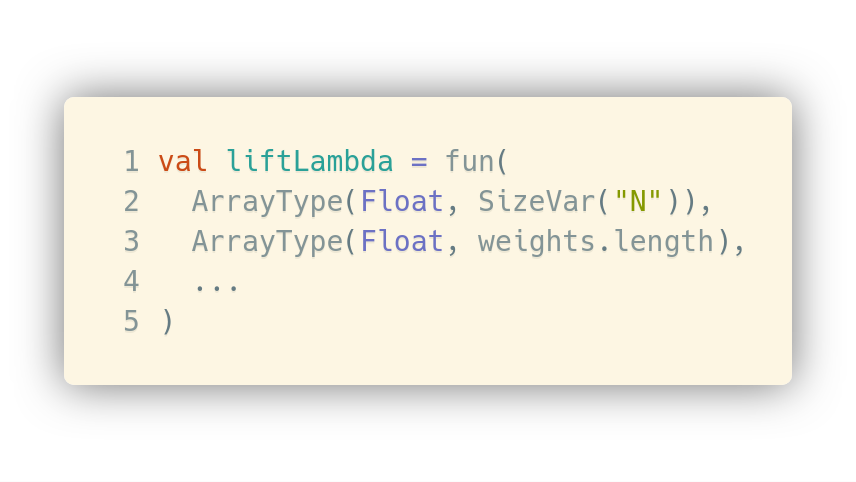
\includegraphics[width=.5\textwidth]{../images/inputData.png}
    \end{center}
\end{block}
    \item Single entry point for arrays into functions  
            \begin{itemize}
                \item Multiple arrays can be zipped together (but must be the same size!) 
            \end{itemize}
            \vspace{-1.5cm}
\begin{block}{}
    \begin{center}
    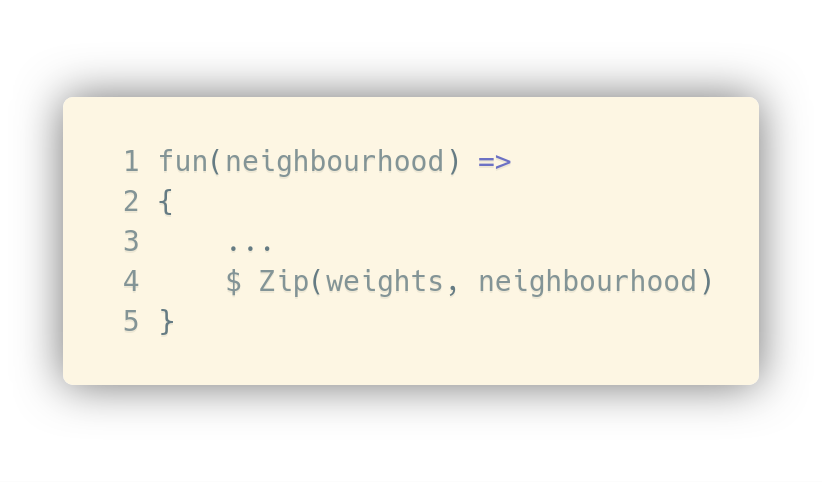
\includegraphics[width=.5\textwidth]{../images/zippedData.png}
    \end{center}
\end{block}
\end{itemize}
\end{frame}

\begin{frame}
\frametitle{Initialising Data in Scala}
\begin{itemize}
    \item Create arrays of data to pass into Lift algorithms in Scala 
        \vspace{-.5cm}
\begin{block}{}
    \begin{center}
         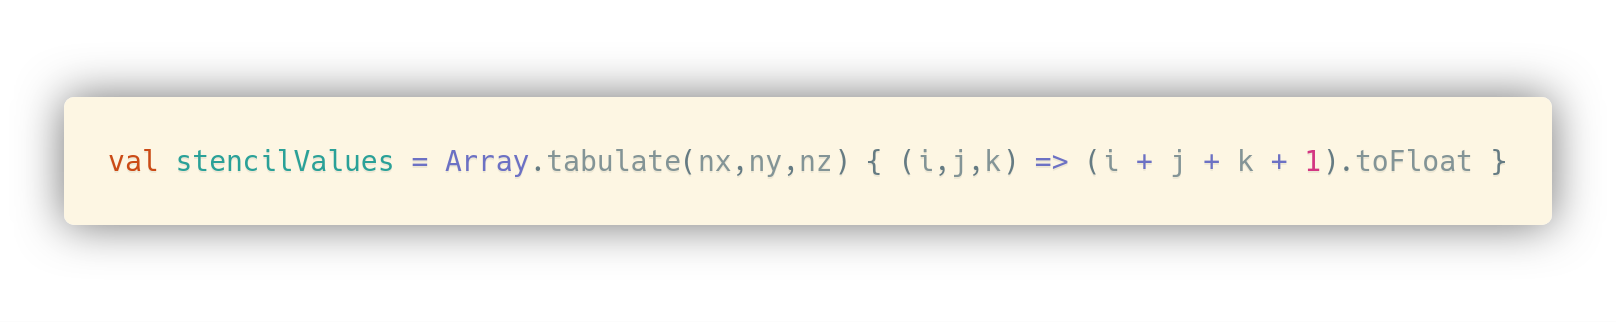
\includegraphics[width=.85\textwidth]{../images/scalaArrays.png}
    \end{center}
\end{block}
    \item Our examples are all in unit tests, which include data to compare against - often from the same algorithm in Scala 
        \vspace{-.5cm}
    \begin{block}{}
        \begin{center}
            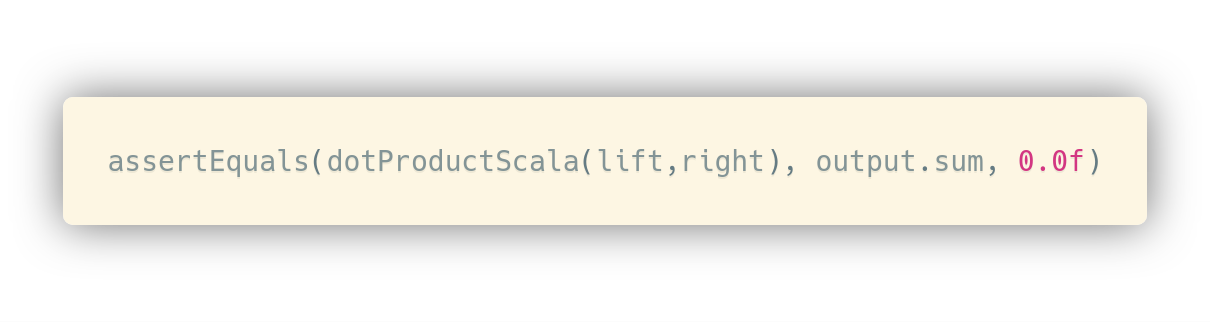
\includegraphics[width=.8\textwidth]{../images/unitTestData.png}
        \end{center}
    \end{block}
\end{itemize}
\end{frame}

\begin{frame}
\frametitle{Developing an Algorithm}
The goal is not for Lift to be programmed in directly.\\
\vspace{.1cm}
However, functionality for new types of algorithms must be added in and tested. In doing so, there are a few things to keep in mind: 
\begin{itemize}
    \item Lift allows multiple inputs, but there is only one data entry point to the main algorithm (can contain tuples)
    \item The algorithm itself must eventually map values back to global memory
    \item The result will be returned in a single array (however, this array can also contain tuples)
\end{itemize}
\end{frame}

\begin{frame}
\frametitle{Simple Example: 1D Jacobi Stencil}
\begin{block}{}
    \begin{center}
    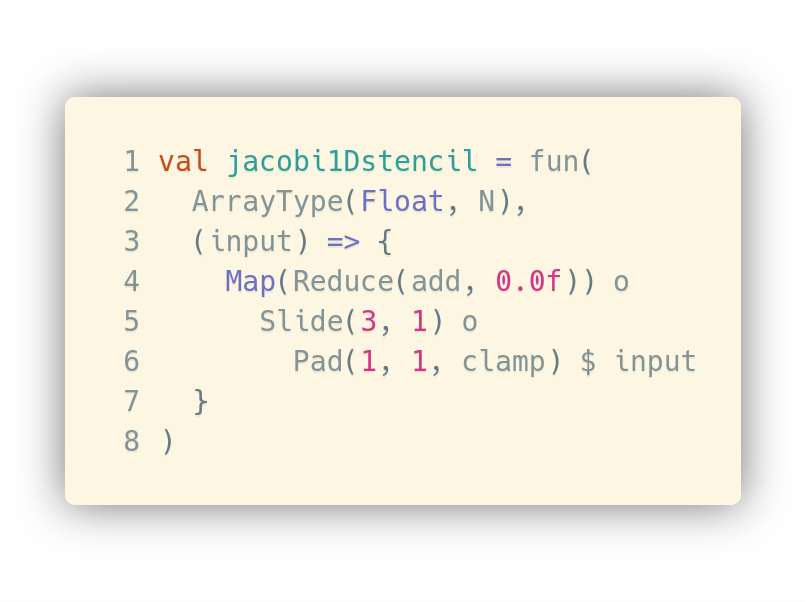
\includegraphics[width=.5\textwidth]{../images/jacobi1Dstencil.png}
    \end{center}
\end{block}
\end{frame}

\begin{frame}
\frametitle{Creating an OpenCL kernel}
\begin{itemize}
    \item To compile your Lift kernel to OpenCL, run \code{[opencl.executor]Compile(<kernel>)}
        \begin{itemize}
                \item This kernel can then be saved as a string or file
        \end{itemize}
        \vspace{-.7cm}
        \begin{block}{}
        \begin{center}
            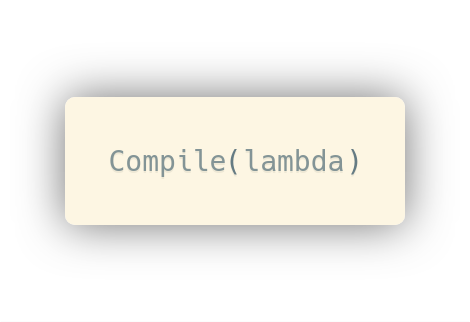
\includegraphics[width=.2\textwidth]{../images/simpleCompile.png}
        \end{center}
        \end{block}
    \item To execute the kernel straight away (compiling will happen behind the scenes), run \code{[opencl.executor]Execute(\textit{<options>})     \\
        \hspace{0.5cm}[Array[\textit{type}]](\textit{lambda}, \textit{..inputs..})}
    \begin{block}{}
        \begin{center}
            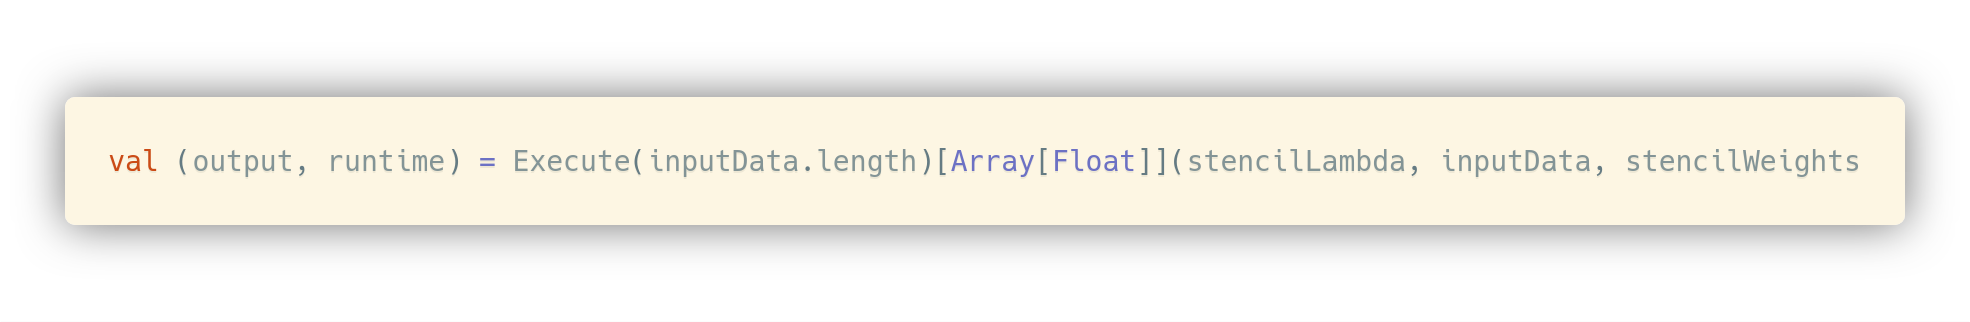
\includegraphics[width=\textwidth]{../images/execute.png}
        \end{center}
    \end{block}
\end{itemize}
\end{frame}



\section{\lift Intermediate Representation}

\begin{frame}
\frametitle{Class diagram}

    \begin{columns}[onlytextwidth]
\begin{column}{0.65\textwidth}
    \vspace{-.5cm}
    \begin{block}{}
        \begin{center}
            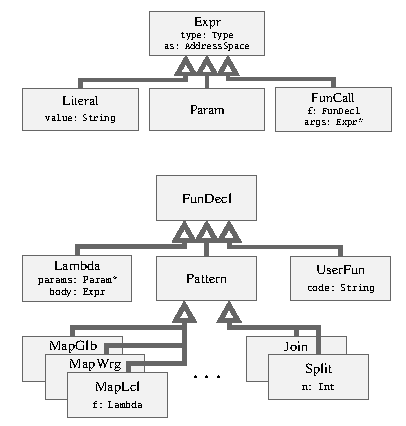
\includegraphics[width=\textwidth]{../images/class_diagram.pdf}
        \end{center}
    \end{block}
\end{column}
\begin{column}{0.35\textwidth}
    \vspace{-.5cm}
\begin{itemize}	
	\item \code{Expressions} represent values and have a type associated with.
\vspace{0.7cm}
	\item \code{Function declarations} represent callable entities: lambdas, patterns and user functions.
\end{itemize}
\end{column}
\end{columns}
\end{frame}

\begin{frame}
\frametitle{Dot product example}
    \vspace{-.8cm}
    \begin{block}{}
        \begin{center}
            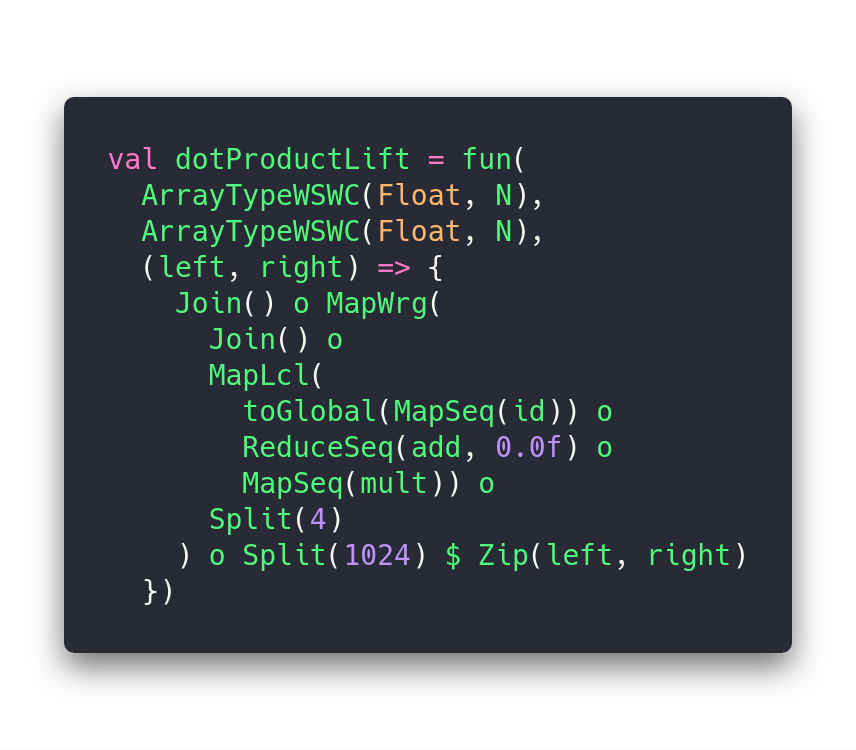
\includegraphics[width=.7\textwidth]{../images/dotProductLift2_expr.png}
        \end{center}
    \end{block}
    \vspace{-.8cm}
        \begin{center}
    For more dot product variations, see \srcurl{src/test/tutorial/applications/DotProduct.scala}
        \end{center}
\end{frame}
%Code

\begin{frame}
\frametitle{Corresponding AST}
    \begin{block}{}
    \vspace{-1cm}
        \begin{center}
            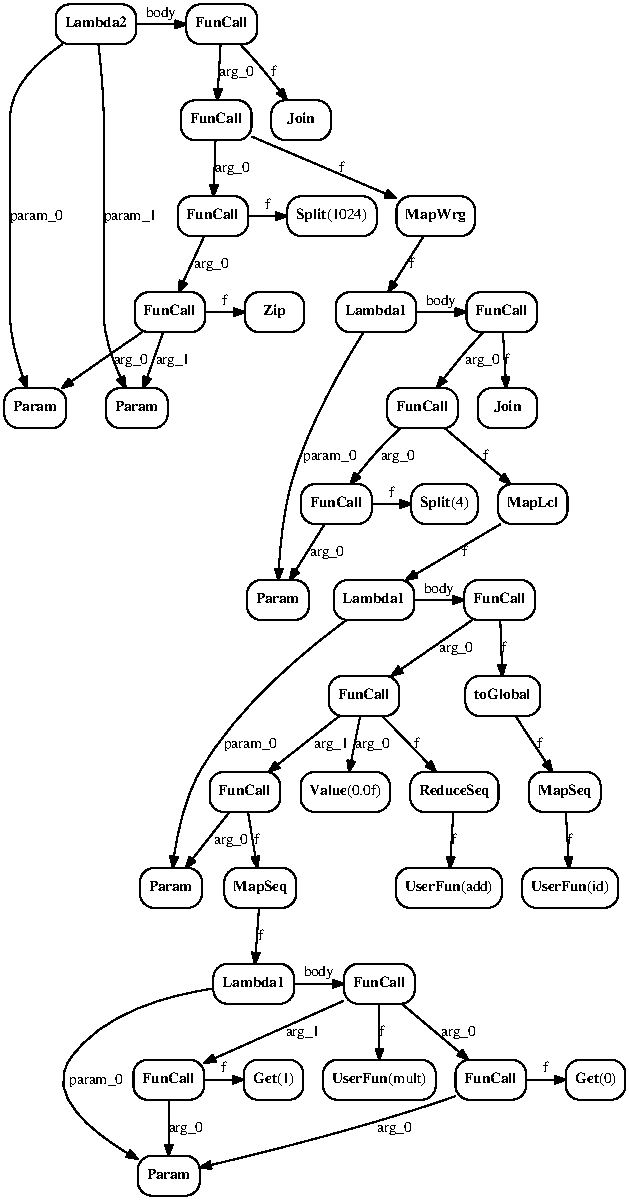
\includegraphics[width=.4\textwidth]{../images/dotProductLift2_ast.pdf}
        \end{center}
    \end{block}
\end{frame}

\section{\lift compilation}

\begin{frame}[t]
\frametitle{Compilation stages}
    \vspace{-1cm}
    \begin{block}{}
        \begin{center}
            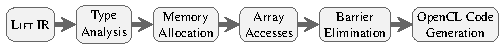
\includegraphics[width=1\textwidth]{../images/compilation_stages.pdf}
        \end{center}
    \end{block}
    \vspace{-0.5cm}
\begin{itemize}
    \item Compile: \srcurl{src/main/opencl/executor/Compile.scala:44}
    \begin{itemize}
    	\item Type checking: \srcurl{src/main/ir/TypeChecker.scala:39}
    	\begin{itemize}
    		\item Example Pattern.checkType(): \srcurl{src/main/opencl/ir/pattern/ReduceSeq.scala:11}
    	\end{itemize}
    	\item Generate: \srcurl{src/main/opencl/generator/OpenCLGenerator.scala:176}
    	\begin{itemize}
    		\item Memory address space inference: \srcurl{src/main/opencl/ir/InferOpenCLAddressSpace.scala:18}
    		\item Domain-specific range inference: \srcurl{src/main/opencl/generator/RangesAndCounts.scala:26}
    		\item Memory allocation: \srcurl{src/main/ir/Type.scala:559}
    		\item Loop unrolling: \srcurl{src/main/opencl/generator/ShouldUnroll.scala:50}
    		\item Barrier elimination: \srcurl{src/main/opencl/generator/BarrierElimination.scala:41}
    		\item Views (array Accesses): \srcurl{src/main/ir/view/View.scala:585}
    	\end{itemize}
    \end{itemize}
\end{itemize}
\end{frame}

\begin{frame}[t]
\frametitle{\lift type system}
    \vspace{-1cm}
    \begin{block}{}
        \begin{center}
            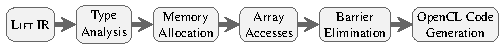
\includegraphics[width=1\textwidth]{../images/compilation_stages.pdf}
        \end{center}
        \vspace{-1.05cm}
        \hspace{1.63cm}
        
\includegraphics[width=1cm, height=0.03cm]{../images/orange_bar.png}
        \vspace{.45cm}
    \end{block}
    \vspace{-0.5cm}
\begin{itemize}
	\item Lift has a \textit{dependent} type system
	\item Scalar types: \code{int}, \code{float}, etc
	\item Vector types corresponding to OpenCL types \code{int2}, \code{float4}, etc
	\item Tuples
	\begin{itemize}
		\item \textit{Represented as \code{structs} in the generated OpenCL code}
	\end{itemize}
	\item Arrays
	\begin{itemize}
		\item Can be nested
		\item Carry information about the size and capacity of each dimension in their type
		\item This information is represented by arithmetic expressions (more on this later)
	\end{itemize}
\end{itemize}
\end{frame}

\begin{frame}[t]
\frametitle{Memory allocation}
    \vspace{-1cm}
    \begin{block}{}
        \begin{center}
            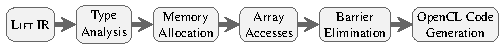
\includegraphics[width=1\textwidth]{../images/compilation_stages.pdf}
        \end{center}
        \vspace{-1.05cm}
        \hspace{3.36cm}
        
\includegraphics[width=1.1cm, height=0.03cm]{../images/orange_bar.png}
        \vspace{.45cm}
    \end{block}
    \vspace{-0.5cm}
\begin{itemize}
	\item The naive approach would be to allocate a new output buffer for every \code{FunCall} AST node
	\item We only allocate memory to the nodes where the called function contains a \code{UserFun}
	\item The address space is inferred from \code{FunCall}
\end{itemize}
\end{frame}

\begin{frame}[t]
\frametitle{Memory allocation}
    \vspace{-1cm}
    \begin{block}{}
        \begin{center}
            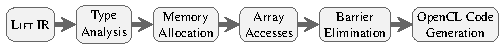
\includegraphics[width=1\textwidth]{../images/compilation_stages.pdf}
        \end{center}
        \vspace{-1.05cm}
        \hspace{3.36cm}
        
\includegraphics[width=1.1cm, height=0.03cm]{../images/orange_bar.png}
        \vspace{.45cm}
    \end{block}
    \vspace{-1.7cm}
    \begin{block}{}
        \begin{center}
            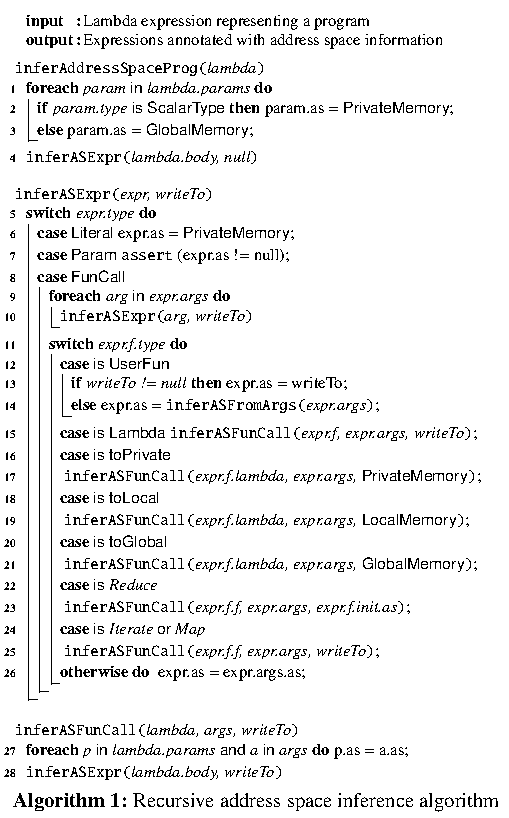
\includegraphics[width=0.47\textwidth]{../images/address_space.pdf}
        \end{center}
    \end{block}
\end{frame}

\begin{frame}[t]
\frametitle{Array accesses}
    \vspace{-1cm}
    \begin{block}{}
        \begin{center}
            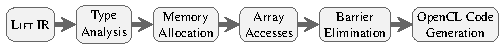
\includegraphics[width=1\textwidth]{../images/compilation_stages.pdf}
        \end{center}
        \vspace{-1.05cm}
        \hspace{5.2cm}
        
\includegraphics[width=.95cm, height=0.03cm]{../images/orange_bar.png}
        \vspace{.45cm}
    \end{block}
    \vspace{-0.5cm}
\begin{itemize}
	\item In \lift IR, arrays are accessed implicitly based on the patterns
	\item This eliminates arbitrary memory accesses and the associated problems
	\item However, expressing (efficient) pattern-transformed accesses is not obvious
	\item ...which is where \code{Views} come to the rescue (but more on that later)
\end{itemize}
\end{frame}

\begin{frame}[t]
\frametitle{Barrier elimination}
    \vspace{-1cm}
    \begin{block}{}
        \begin{center}
            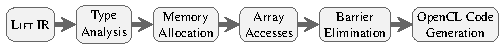
\includegraphics[width=1\textwidth]{../images/compilation_stages.pdf}
        \end{center}
        \vspace{-1.05cm}
        \hspace{6.9cm}
        
\includegraphics[width=1.25cm, height=0.03cm]{../images/orange_bar.png}
        \vspace{.45cm}
    \end{block}
    \vspace{-0.5cm}
\begin{itemize}
	\item We start by synchronizing after each occurrence of a parallel \code{Map}
	\item Then we remove barriers one by one in cases when it can be inferred that they are not required
	\begin{itemize}
		\item When the data is not shared (i.e. \code{Split}, \code{Join}, \code{Gather} and \code{Scatter} are not used)
		\item When the two parallel \code{Maps} are executed independently in separate branches of \code{Zip}
	\end{itemize}
\end{itemize}
\end{frame}

\begin{frame}[t]
\frametitle{OpenCL code generation}
    \vspace{-1cm}
    \begin{block}{}
        \begin{center}
            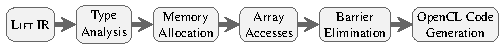
\includegraphics[width=1\textwidth]{../images/compilation_stages.pdf}
        \end{center}
        \vspace{-1.05cm}
        \hspace{8.9cm}
        
\includegraphics[width=1.57cm, height=0.03cm]{../images/orange_bar.png}
        \vspace{.45cm}
    \end{block}
    \vspace{-0.5cm}
\begin{itemize}
	\item The AST is traversed recursively
	\item No OpenCL code is generated for the patterns that only affect \code{View}
	\item Low-level optimizations such as loop unrolling are applied to simplify the control flow using the information on \textit{ranges} inferred from the patterns such as \code{mapLcl}
\end{itemize}
\end{frame}

\begin{frame}
\frametitle{The end}
\begin{center}
Slides are available at
\textcolor{blue}{\url{http://www.lift-project.org/ispass2018}}
\end{center}
\end{frame}

\end{document}
